\subsection{Rising Velocity or drag force}

\begin{itemize}
    \item Include Ridcharson - Zaki correlation (Ahmadi 2021)
    \item Surface averaged velocity  ???  $\avg{\textbf{u}_I\delta_I}$
    \item Look at \citet{jackson2000dynamics} and \citet{wang2021numerical} to introduce the drag force term. 
\end{itemize}

\begin{figure}[h!]
    \centering
    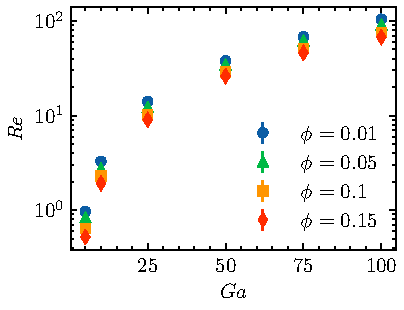
\includegraphics[height = 0.3\textwidth]{image/HOMOGENEOUS/fCA/Re.pdf}
    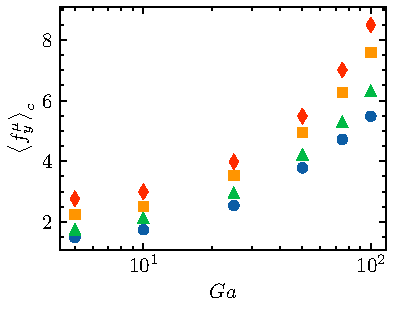
\includegraphics[height = 0.3\textwidth]{image/HOMOGENEOUS/fCA/FH_mu_Ga.pdf}
    \caption{(left) Reynolds number based on the averaged rising velocity.
    (right) Dimensionless drag force.}
\end{figure}